\documentclass[11pt,spanish]{article} % Idioma
\usepackage{babel}
\usepackage[T1]{fontenc}
\usepackage{textcomp, verbatim} % \begin{comment}
\usepackage[utf8]{inputenc} % Permite acentos

\usepackage{wrapfig} % Imagenes %\graphicspath{ {./imagenes/} }
\usepackage[left=2.75cm,top=2.5cm,right=2cm,bottom=2.5cm]{geometry} % Márgenes
\usepackage{amssymb, amsmath, amscd, amsfonts, amsthm, mathrsfs } % Símbolos matemáticos
\usepackage{cancel} % Cancelar expresiones
\usepackage{multirow, multicol, tabularx, booktabs, longtable} % Tablas
\usepackage{fancyhdr, fncychap} % Encabezados
\usepackage{algpseudocode, algorithmicx, algorithm} % Pseudo-código	
\usepackage{bbding} % Símbolos
\usepackage{enumitem} % Enumerados a), b), c)... usando \begin{enumerate}[label=\alph*)]
\usepackage{graphicx, xcolor, color, pstricks} % Gráficos --TikZ-- 
% http://www.texample.net/tikz/examples/
\usepackage[hidelinks]{hyperref}  % Enlaces
\usepackage{verbatim} % Comentarios largos \begin{comment}
\usepackage{rotating} % \begin{rotate}{30}
\usepackage[all]{xy} % Diagramas
\usepackage{xparse} % Entornos
\usepackage{listings}

\definecolor{codegreen}{rgb}{0,0.6,0}
\definecolor{codegray}{rgb}{0.5,0.5,0.5}
\definecolor{codepurple}{rgb}{0.58,0,0.82}
\definecolor{backcolour}{rgb}{0.95,0.95,0.92}

\lstdefinestyle{mystyle}{
	backgroundcolor=\color{backcolour},   
	commentstyle=\color{codegreen},
	keywordstyle=\color{magenta},
	numberstyle=\tiny\color{codegray},
	stringstyle=\color{codepurple},
	basicstyle=\footnotesize,
	breakatwhitespace=false,         
	breaklines=true,                 
	captionpos=b,                    
	keepspaces=true,                 
	numbers=left,                    
	numbersep=5pt,                  
	showspaces=false,                
	showstringspaces=false,
	showtabs=false,                  
	tabsize=2
}
\lstset{style=mystyle}


% Comandos
\newcommand{\docdate}{}
\newcommand{\subject}{}
\newcommand{\docauthor}{Rubén Morales Pérez}
\newcommand{\docemail}{srmorales@correo.ugr.es}

\newcommand{\N}{\mathbb{N}}
\newcommand{\Q}{\mathbb{Q}}
\newcommand{\C}{\mathbb{C}}
\newcommand{\R}{\mathbb{R}}
\newcommand{\Z}{\mathbb{Z}}




\usepackage[final]{pdfpages}


\linespread{1.1}                  % Espacio entre líneas.
\setlength\parindent{0pt}         % Indentación para párrafo.

\title{INGENIERÍA DE REQUISITOS \\
	Modelo de casos de uso}
\author{Alicia Rodríguez Gómez \\
	Francisco Javier Morales Piqueras \\
	Rubén Morales Pérez \\
	Samia Mikou}
\date{\today}

% % % % % % % % % % % % % % % % % % % % % % % % % % % % % % % % %
%					 Inicio del documento
% % % % % % % % % % % % % % % % % % % % % % % % % % % % % % % % %
\begin{document}

\maketitle
\tableofcontents % Generando el indice
\setlength\parindent{0pt} % Quitamos la sangría

\vspace{5cm}
\section{Introducción}
En este documento se exponen los diferentes diagramas de uso  para el sistema “Tapuntas”. Veremos una descripción de todos los casos de uso, junto con un glosario de términos.

\setboolean{@twoside}{false}


\section{Diagramas realizados por Francisco Javier Morales Piqueras}

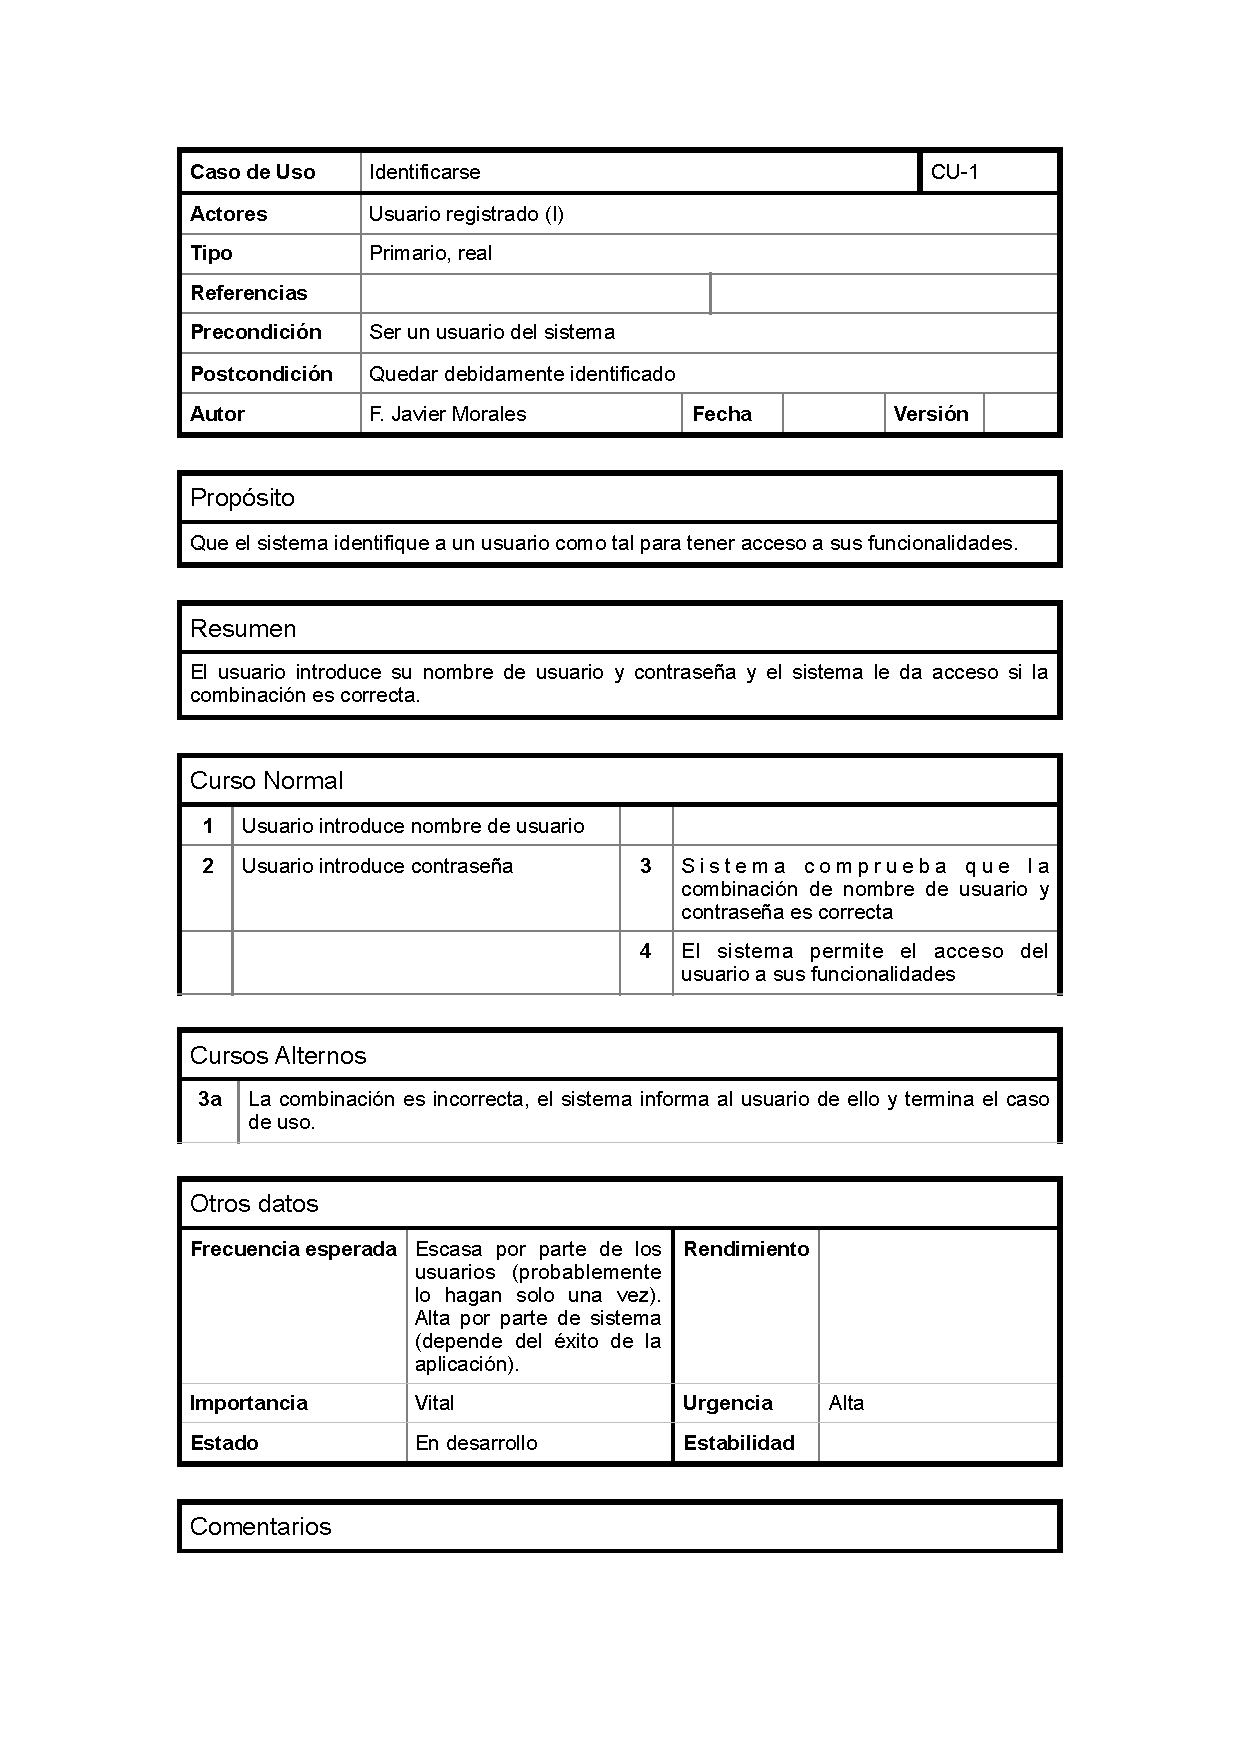
\includepdf[pages=-]{./pdf's/FraJavMorPiq.pdf}
\newpage


\section{Diagramas realizados por Rubén Morales Pérez}

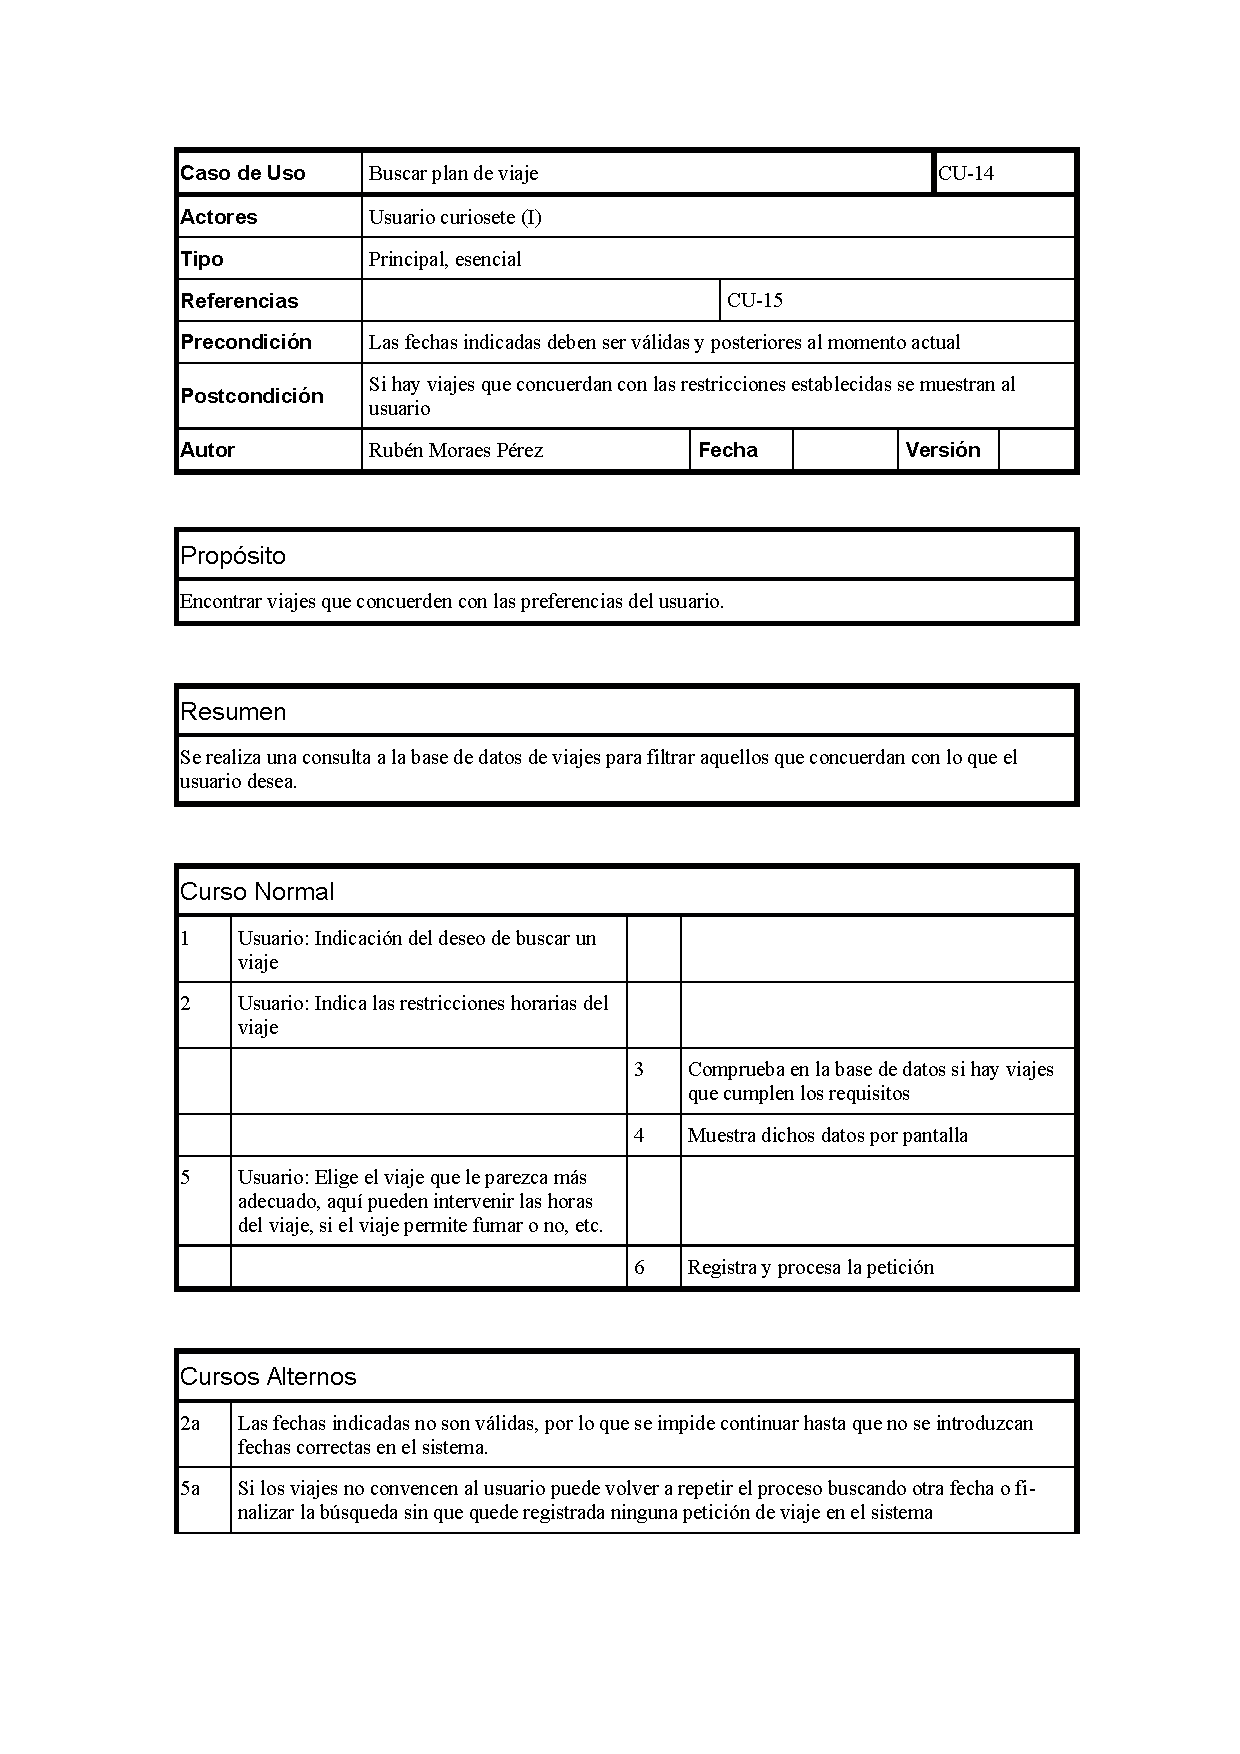
\includepdf[pages=-]{./pdf's/RubMorPer.pdf}
\newpage

\section{Diagramas realizados por Alicia Rodríguez Gómez}

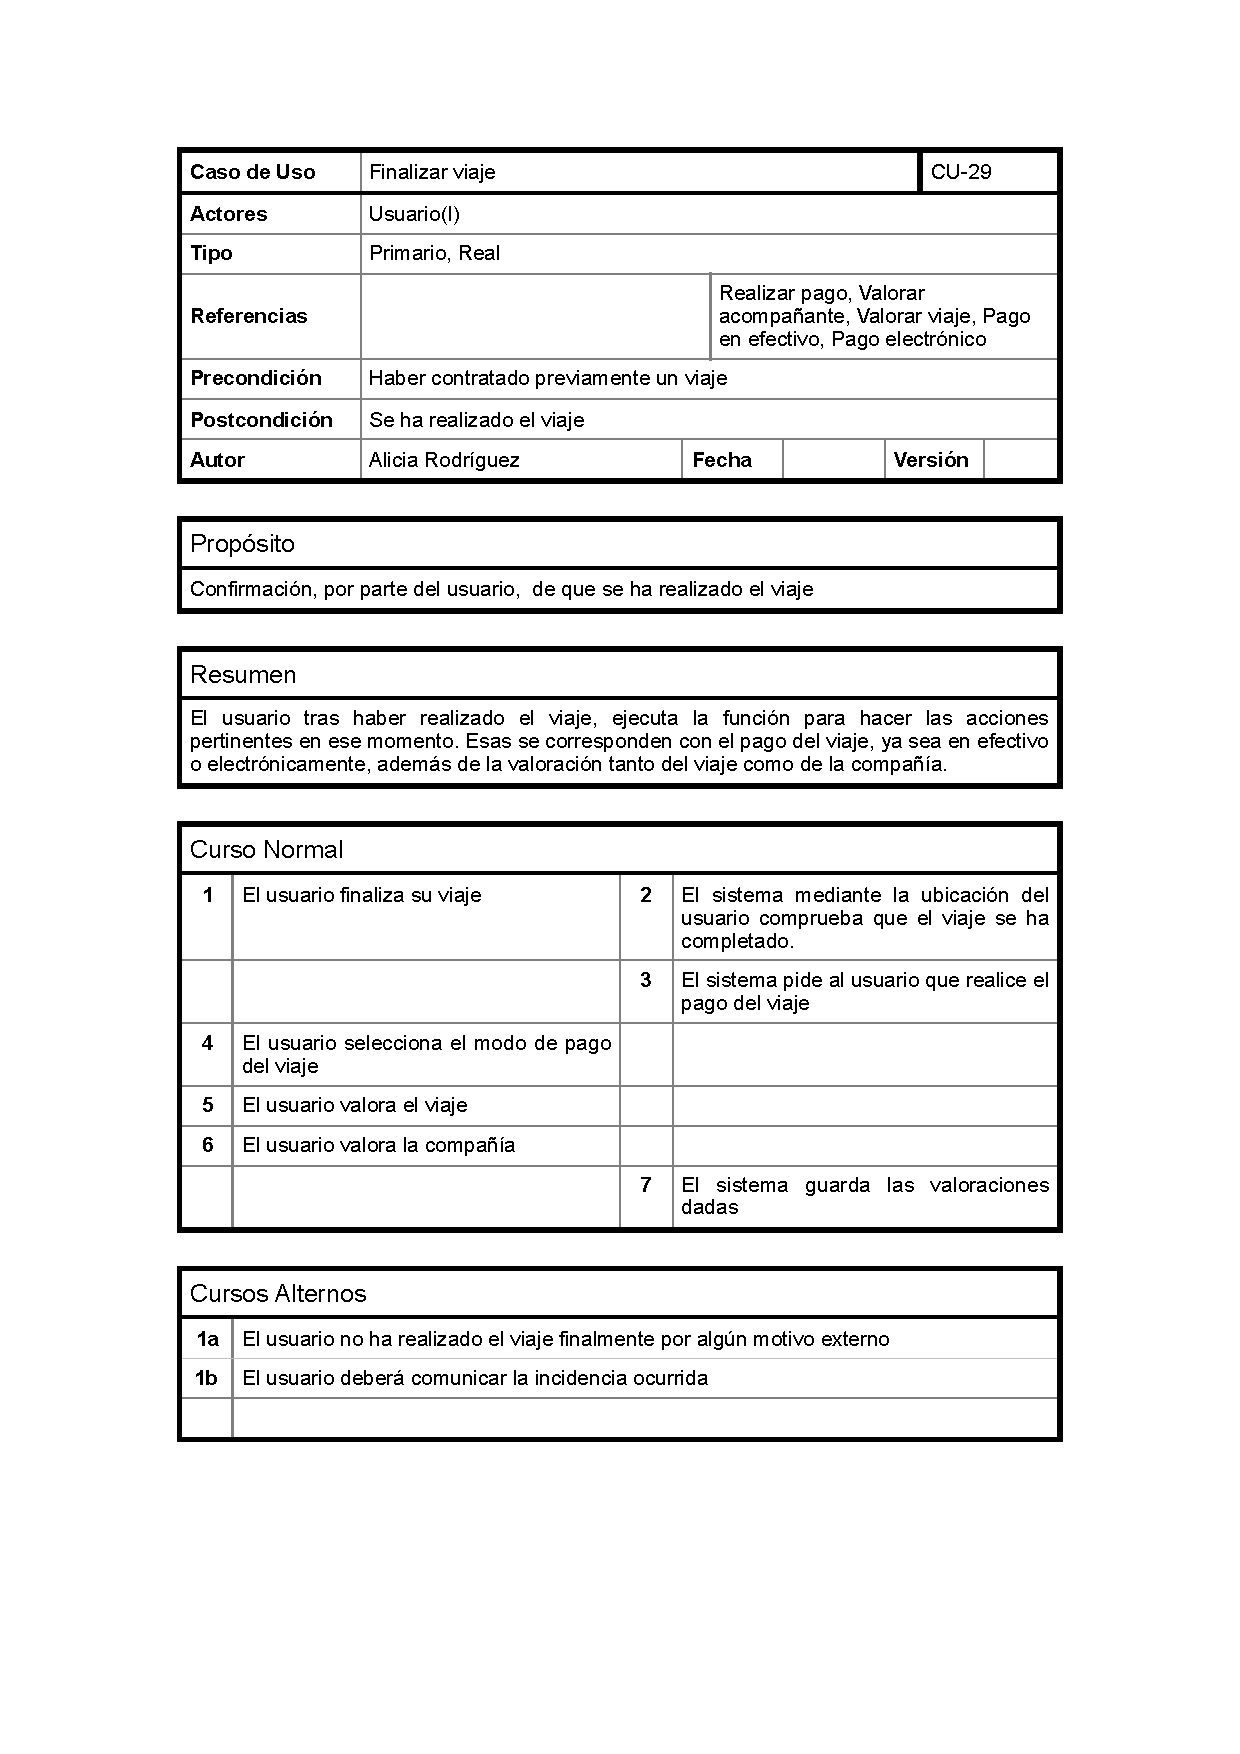
\includepdf[pages=-]{./pdf's/Alicia.pdf}
\newpage

\section{Diagramas realizados por Samia Mikou}
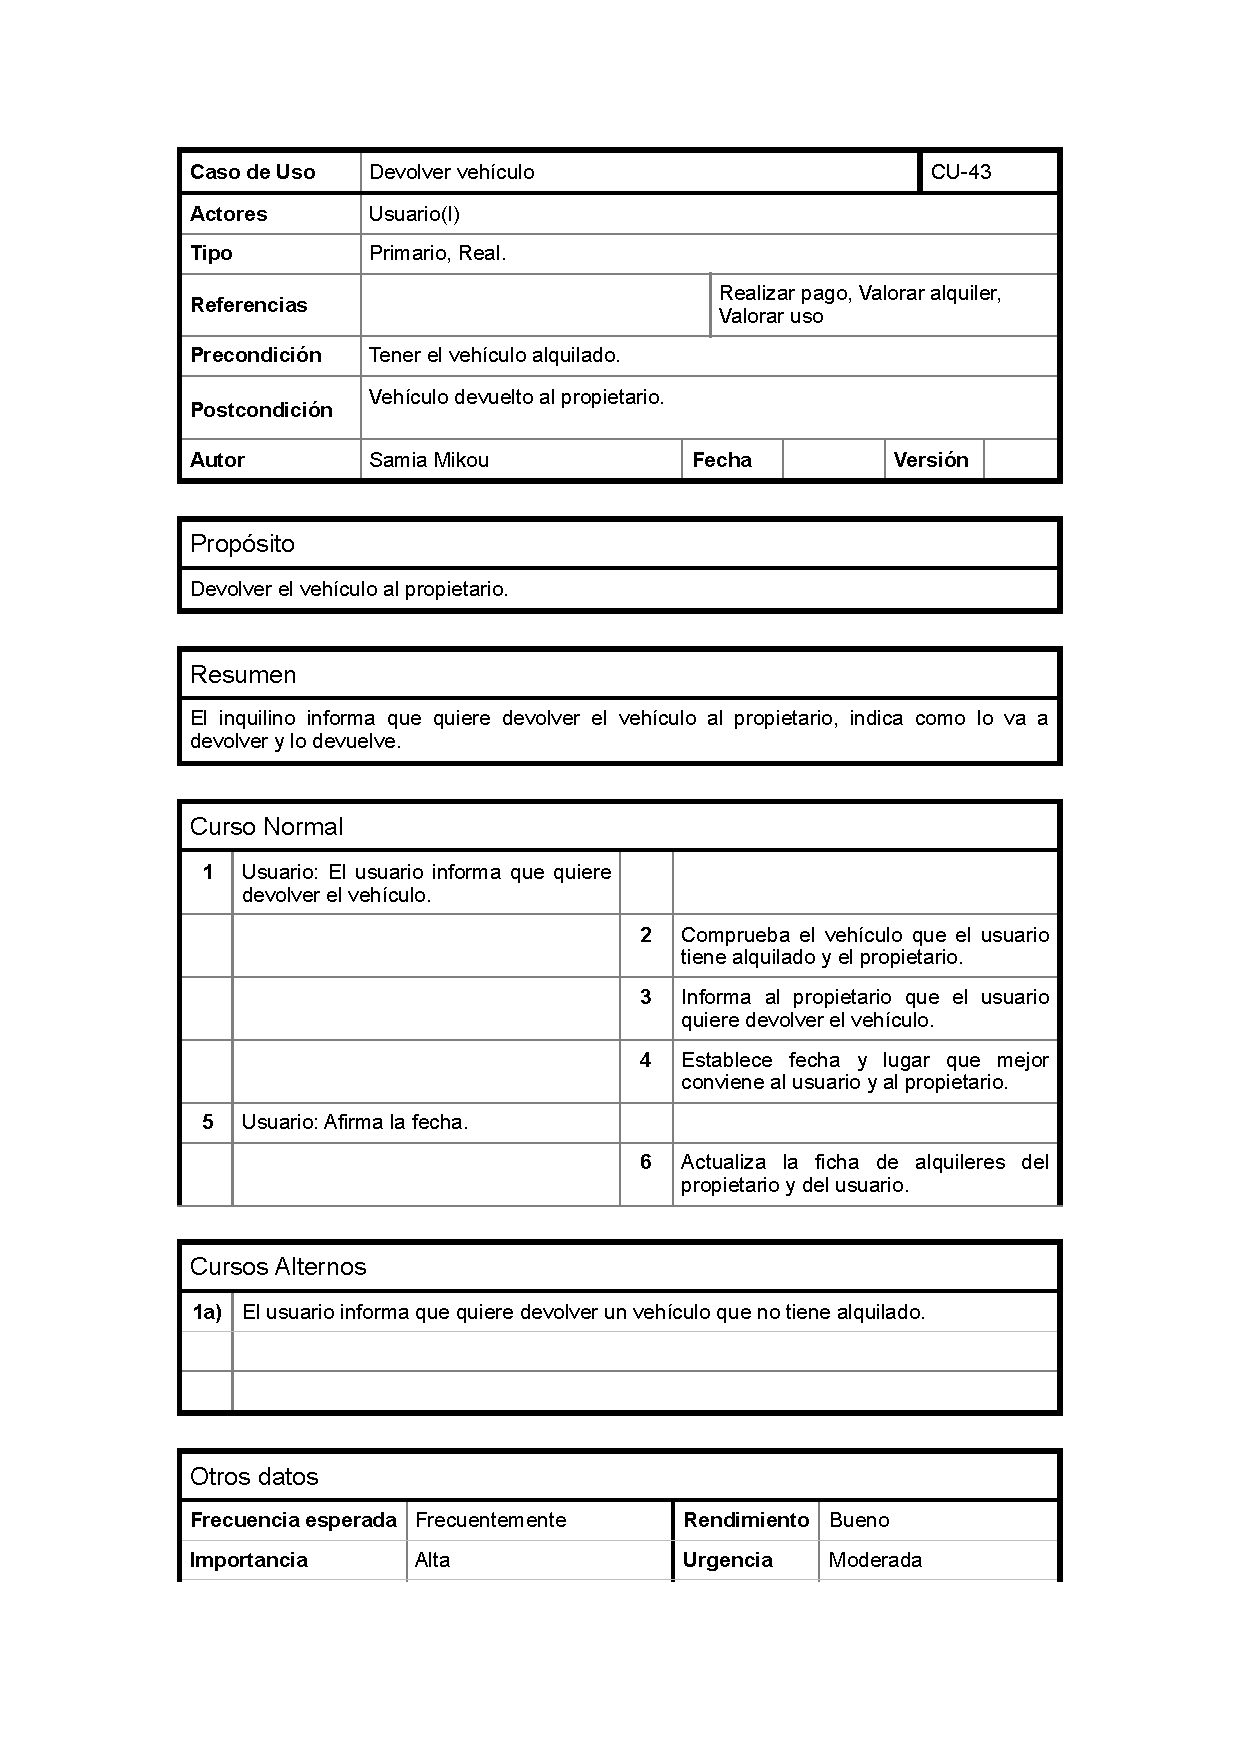
\includepdf[pages=-]{./pdf's/Samia.pdf}
\newpage

\section{Glosario de términos}
\begin{itemize}
	\item Valoración: Puntuación numérica entre 0 y 5 (incluidos), donde 0 es la menor calificación y 5
la mayor.
	\item Economía colaborativa: Interacción entre dos o más sujetos, a través de medios digitalizados o
no, que satisface una necesidad real o potencial, a una o más personas.
	\item Saldo virtual : Dinero ficticio asociado a cada usuario que puede obtener al beneficiarse de alqui-
leres (también podemos canjearlo por alquileres) y puede transferirse a una cuenta bancaria.
	\item Status: Nivel del usuario dentro de la plataforma, que se modifica en función de la experiencia
y las opiniones recibidas de otros usuarios.
	\item Subtrayecto: Trayecto parcial del viaje, que empieza y/o acaba en paradas intermedias.
	\item Pago electrónico: sistema de pago que facilita la aceptación de pagos electrónicos para las transacciones en línea a través de internet.
	\item Plan de viaje: Itinerario que se realizará durante el viaje
\end{itemize}


%%%%%%%%%%%%%%%%%%%%%%%%%%%%%%%%%%%%%%%%%%%%%%%%%%%%%%%%%%%%%%%%%%%%%%%%%%%%%%%%%%




\end{document}
